\documentclass[tikz, border=3.14mm]{standalone}
\usepackage{pgfplots}
\pgfplotsset{compat=1.18}
\usepgfplotslibrary{groupplots}

\begin{document}
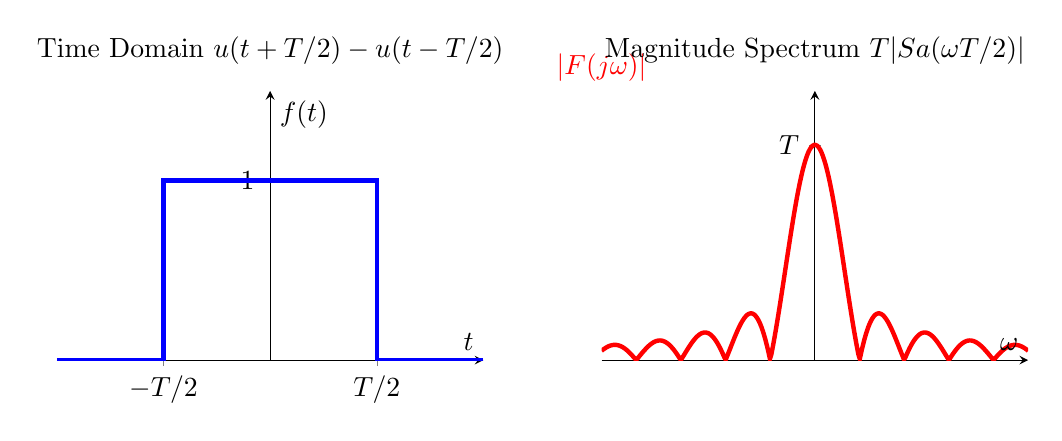
\begin{tikzpicture}
    \begin{groupplot}[
        group style={group size=2 by 1, horizontal sep=1.5cm},
        axis lines = middle,
        width = 7cm, height = 5cm,
        grid=none,
        xlabel = {$t$},
        ylabel = {$f(t)$}
    ]
        % Time Domain Rectangular Pulse
        \nextgroupplot[
            title = {Time Domain $u(t+T/2)-u(t-T/2)$},
            xmin = -2, xmax = 2,
            ymin = 0, ymax = 1.5,
            ytick = {1},
            yticklabels = {$1$},
            xtick = {-1, 1},
            xticklabels = {$-T/2$, $T/2$}
        ]
        \draw[ultra thick, blue] (-2,0) -- (-1,0) -- (-1,1) -- (1,1) -- (1,0) -- (2,0);

        % Frequency Domain Sampling Function
        \nextgroupplot[
            title = {Magnitude Spectrum $T|Sa(\omega T/2)|$},
            xlabel = {$\omega$},
            ylabel = {$|F(j\omega)|$},
            ylabel style={at={(axis description cs:0,1)},anchor=south, red},
            xmin = -15, xmax = 15,
            ymin = 0, ymax = 2.5,
            ytick = {2},
            yticklabels = {$T$},
            samples = 300,
            xtick = \empty
        ]
        \addplot[ultra thick, red, domain=-15:15] {2 * abs(sin(deg(x))/x)}; 
        % T=2, omega*T/2 = x. Resulting peak is T=2.
        \node[anchor=north] at (axis cs:3.14, 0) {$\frac{2\pi}{T}$};
        \node[anchor=north] at (axis cs:-3.14, 0) {$-\frac{2\pi}{T}$};

    \end{groupplot}
\end{tikzpicture}
\end{document}
